\subsection{The extension on the full corpus}
\label{sec:res-extension}

% generated by scripts/make_numbers.py; do not edit
\begin{table}[t]
\centering
\caption{The extension's own run over the full corpus against the recorded results of the research implementation. $^\dagger$Reactions with a chemical value from measurement or Hess's law. $\ast$~Differs; see text.}
\label{tab:reproduction}
\footnotesize
\begin{tabular*}{\columnwidth}{@{\extracolsep{\fill}}lrr@{}}
\toprule
Quantity & Research & Extension \\
\midrule
Internal species & 5{,}330 & 5{,}330 \\
Rank of $N$ & 2{,}667 & 2{,}667 \\
Conservation laws & 2{,}663 & 2{,}663 \\
Steady-state flux modes & 247 & 247 \\
Blocked, medium open & 2{,}364 & 2{,}364 \\
Blocked, boundary open & 95 & 95 \\
Measured \DG: answered & 75 & 75 \\
\quad refused & 2{,}244 & 2{,}244 \\
\quad absent & 595 & 595 \\
Hess's law: answered & 30 & 30 \\
\quad absent & 367 & 367 \\
\quad certified empty & 1 & 1 \\
Hess fit: $\chi^2$ / degrees of freedom & 275.6 / 67 & 275.6 / 67 \\
Species state: absent & 4{,}603 & 4{,}603 \\
\quad underdetermined & 727 & 727 \\
Direction$^\dagger$: answered & 2 & 10\,$\ast$ \\
\quad concentrations decide & 60 & 52\,$\ast$ \\
\quad medium decides & 43 & 43 \\
\bottomrule
\end{tabular*}
\end{table}


\paragraph{Reproduction}
The research implementation prepared the inputs: the corpus, the ChEBI-to-KEGG mapping, the TECRDB rows and the microspecies table.
Everything computed from them was computed by the extension's own code, which shares no code with the research implementation at run time.
Over the 2{,}914 reactions it answered \xVerdicts\ questions, and every structural and thermodynamic count equals the recorded result, including the rank, the blocked reactions, the Hess span and the $\chi^2$ of the Hess fit (\cref{tab:reproduction}).
The singular value decompositions took about \xStructureMin\,min.

The directions differ as intended.
The extension answers \xDirAnswered\ directions where the research implementation answered \xDirKernel.
They are the \xDirAnsweredMeasured\ pyrophosphate hydrolyses and \xDirAnsweredHess\ hydrolyses of cyclic AMP by phosphodiesterases, whose \DG\ comes from Hess's law.
Evaluating the concentration term at 298.15\,K instead of 310\,K narrows $RT\ln Q$ by 4\%, enough to decide these \xDirAnsweredHess\ reactions, which a sensitivity analysis of the research implementation had predicted.
They clear zero by \xMarginHess\kJ; crowding cannot move them, because they conserve the number of solute particles, but the choice of temperature does.
The pyrophosphate hydrolyses now clear zero by \xMarginMeasured\kJ, still less than the \xCrowding\kJ\ crowding shift at $a=0.7$, so M3a would fail again.
For \xDirConc\ of the other reactions the sign of \DGm\ is fixed and concentrations decide, and for \xDirMedium\ the medium window decides.

\paragraph{Catalogue}
The emitted dataset has \xTriples\ triples in five named graphs (\cref{fig:extension}a), \xTrigMB\,MB as TriG.
The stated graph holds \xStated\ triples and the derived graph \xDerived, one verdict for each of the \xVerdicts\ questions and \xGibbs\ Gibbs energies with unit and uncertainty.
The supplied and provenance graphs are small: the medium, \xConventions\ conventions and one run.
Emission took \xEmit\,s, serialisation \xSerialise\,s and SHACL validation \xValidate\,s, and the catalogue conforms with no validation result.
Across corpus prefixes from \xScalingMin\ to \xTriples\ triples, validation time grows as the \xScalingSlope\ power of the number of triples (\cref{fig:extension}b).

Every empty or absent result in the catalogue carries an absence code: \xGateNotRecorded\ not recorded, \xGateOpen\ unmappable, \xGateWitnessed\ witnessed and \xGateUndecided\ undecided.
The undecided codes all belong to species states, whose blockers (missing rate constants, equilibrium constants and concentrations) have no entry in the rule table yet; the code exposes this gap instead of hiding it.

\paragraph{Shapes}
On the catalogue of the bundled example (\xControlTriples\ triples), validation reports nothing for the unaltered graph and catches each of \xControlCaught\ planted defects (\cref{fig:extension}c).
A payload on a non-answer (V1), a removed blocker (V2), an absence code on an answer and a supplied basis without a convention each violate one disjunctive constraint of the verdict shape.
A status label outside the vocabulary also violates the enumeration, and a malformed stage digest violates its pattern.

\paragraph{Comparing runs}
A second run used a narrower medium (pH \xNarrowPh, ionic strength \xNarrowI\,M, pMg \xNarrowPmg), so its conventions digest differs from the first.
Both runs minted the same \xShared\ verdict IRIs.
One SPARQL query over the two derived graphs joined them in \xJoinMs\,ms and found \xChanged\ changed verdict: the direction of \xChangedReaction\ became forward (\cref{fig:extension}d).
A medium window four times narrower in pH thus decides one further direction, which supports M2b: the binding constraint is concentrations, not the medium.

\paragraph{Files}
The \xParquetRows\ verdicts were written as a table with \term{CircuitDataset} metadata to a Parquet file of \xParquetKB\,kB through SciDatS.
SciDatS dispatched the metadata to the extension's profile, read the table back unchanged and restored the metadata class, and no network connection was attempted.
Writing took \xParquetWrite\,s, including the first load of the profile's schema, and reading \xParquetRead\,s.

\begin{figure*}[t]
\centering
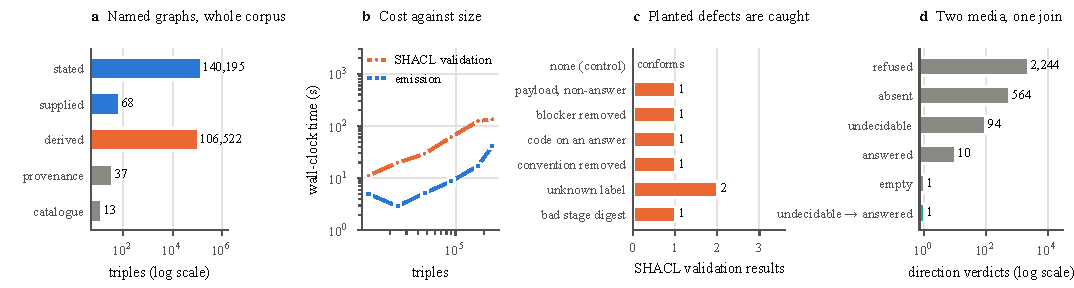
\includegraphics[width=\textwidth]{figures/fig_extension.pdf}
\caption{The DCAT-AP-PLUS extension on the full corpus.
(a) Triples per named graph of the emitted catalogue (log scale); blue graphs record the stated and supplied basis, orange the derived verdicts.
(b) Wall-clock time of emission and SHACL validation against the number of triples, for corpus prefixes and the full corpus.
(c) Validation results for the unaltered catalogue of the bundled example (the control) and for six planted defects.
(d) Direction verdicts of two runs under different media, joined on verdict IRIs with one SPARQL query; each bar is a pair of status labels (first run $\to$ second run), and the green bar is the only pair that changed.}
\label{fig:extension}
\end{figure*}
